\chapter{Related Work}
This chapter explains the previous work and concepts which led to the development of the synchronization component in the KIA4SM project. It explains the synchronization algorithms available and provides the results of a comparative study of these algorithms.  

\section{Synchronization of L4 Fiasco.OC tasks}

The thesis is largely based on the work of Robert H{\"a}cker, who in his bachelor thesis \textit{ "Design of an OC-based Method for efficient Synchronization of L4 Fiasco.OC Mircrokernel Tasks"} \cite{haecker}, describes the design of a scheduler best suited for the  KIA4SM project. He also gives a comparison study of the different schedulers and the synchronization methods suited for updating the task ready queue. 

He suggests the Modified-Maximum-Urgency-First(MMUF) algorithm as the best choice for the KIA4SM project due to the importance of safety and security in embedded systems. After comparing the synchronization algorithms, the sequential lock technique was chosen to be the best since it offers better control. Another option that he suggested is the Read-Copy Update(RCU) algorithm. However, both these methods are untested. 

This work is an extension of H{\"a}cker's findings. However, the focus of the thesis is to develop a good synchronization method without the implementation of a scheduler.

Some of the ideas and code knowledge were taken from Valentin Hauner's bachelor's thesis \textit{"Extension of the Fiasco.OC microkernel with context-sensitive scheduling abilities for safety-critical applications in embedded systems"} \cite{hauner}. In his thesis, he added the EDF scheduling strategy. Though his thesis concentrated on using it in the L4RE environment, it provided a good starting point for this thesis.

\section{Synchronization Methods} \label{rq:sync}
This section describes the synchronization methods that were studied in this thesis. The synchronization methods are categorized based on the techniques that they use to provide concurrent access. The figure \ref{fig:sync} shows the different types of synchronization methods along with examples. 
\begin{figure}[h]
\centering
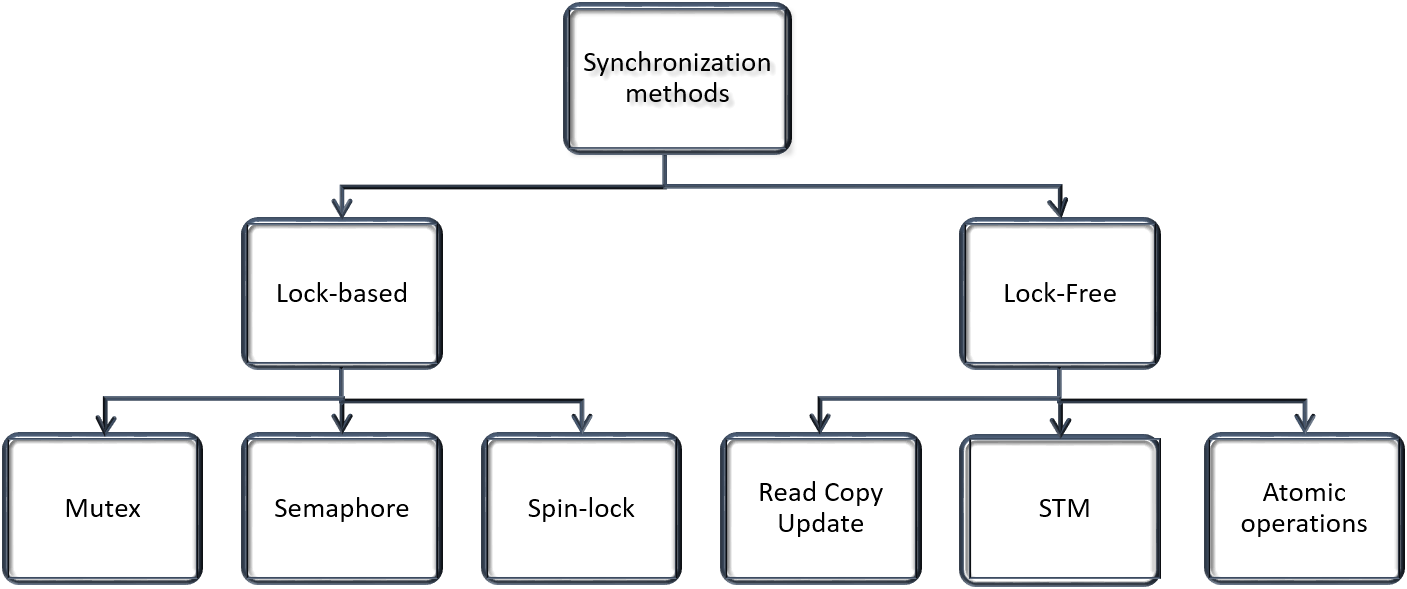
\includegraphics[width=0.9\linewidth]{figures/sync}
\caption{Lock-free and lock-based synchronization methods}
\label{fig:sync}
\end{figure}


\subsection{Lock Based Algorithms}
Lock based algorithms are a simple way of enforcing the limits on access to shared resources, when there are multiple threads of execution. A lock enforces a mutual exclusion concurrency control. The code region where the read or write is happening to a shared resource is called a critical section. A thread has to acquire a lock before entering the critical section and only one thread can acquire this lock. Whenever it leaves the critical section, the thread should release the lock so that the other threads can enter the critical section.

Some of the lock-based synchronization methods are,

\begin{labeling}{lock}
\item[Mutex] Mutex is a synchronization primitive that stands for mutual exclusion, which prevents the simultaneous access to the shared resource. The thread, which wants to execute in a critical section has to acquire the mutex. Once finishes the execution in the critical section, it has to release the mutex. 

\item[Semaphore] It is a variable that is used to control the common resource access between multiple processes/threads. A typical semaphore is initialized with an initial value equal to the number of resources  available and the value is decremented whenever a process takes the resource. If the value of the semaphore is 0, then all the resources are empty and the thread/process has to wait. This works in the opposite way for event management, where the initial value is 0 and the semaphore is increased every time an event occurs and decremented when the corresponding event is processed. A binary semaphore has only two values (0 and 1) and works similar to a mutex.   

\item[Spin-lock] It is a type of lock, where the thread that wants to access the critical section waits in a loop (spin) while trying to acquire the lock. The thread remains active on the CPU while no useful work is being done. Spin locks have a very good advantage if the threads are blocked for shorter periods of time.
\end{labeling} 

The lock-based synchronization primitives are simple and easy to implement. However, there exist a lot of disadvantages. If the programmer is not careful, deadlocks can occur, which are difficult to debug. One interesting problem that might arrive is priority inversion, which is defined for two threads i and j as, if J is in a critical section, assign J the highest priority and when it exits the critical section, assign its original priority. The problem with priority inversion is that a higher priority thread has to wait for the lower priority thread. This is not desirable for real time systems. Another problem is thread starvation, where a thread doesn't get CPU time due to long waits.
 
\subsection{Lock-Free Algorithms}

Lock-Free algorithms refer to a synchronization method where the access to critical section for all the threads is guaranteed without using the locks. Two major algorithms are discussed in the category of lock free algorithms.

\textbf{Read-Copy Update:}
Read-Copy Update (RCU) guarantees concurrent read and write operations to the same data.  It is a synchronization mechanism that was added to the Linux kernel during the 2.5 development effort and is optimized for read-mostly situations. RCU achieves scalability improvements by allowing reads to occur concurrently with updates \cite{whatisrcu}. Compared to conventional locking primitives, which ensure mutual exclusion among concurrent threads regardless of read/write operation, RCU supports concurrency between single updater and multiple readers. This is achieved in RCU by keeping multiple versions of variables and ensuring that they are not freed until all the pre-existing readers have finished using the old copies of the variable. RCU uses three main mechanisms to achieve lock-free synchronization method, which are,

\begin{labeling}{rcumethods}
\item[\textbf{Publish-Subscribe Mechanism (for insertion)}:]
Publish-subscribe mechanism is a way of enforcing the compiler to execute the instructions in the correct order. If a pointer is getting updated, an RCU call(rcu\_assign\_pointer())  is used to change the pointer. This can be thought of as publishing the data. This requires that the readers wait for the update to happen to read the correct data and the dereferencing of the pointer is done by using an RCU call(rcu\_dereference()), which is further guarded by RCU read lock.

\item[\textbf{Wait For Pre-Existing RCU Readers to Complete (for deletion)}:]
The figure \ref{fig:rcu_grace} shows RCU's way of waiting for pre-existing reader threads to finish. RCU introduces a grace period where it waits on a read-side critical section. The simple way to find out when the reader threads have finished executing the critical section is to check for the context switch of the CPU. 

\begin{figure}[h]
\centering
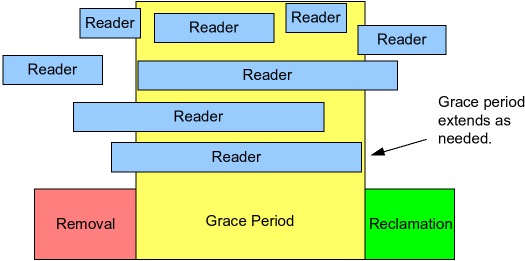
\includegraphics[width=0.7\linewidth]{figures/rcu_grace}
\caption{RCU showing the usage of grace period \cite{whatisrcu}}
\label{fig:rcu_grace}
\end{figure}

\item[\textbf{Maintain Multiple Versions of Recently Updated Objects (for readers)}]:
RCU maintains multiple versions of the data in between the removal and the reclamation phases. The figure \ref{fig:rcu} shows how RCU maintains these multiple versions of data. In the linked list, node B has to be removed. The first phase is changing the link from A to C, but the link from B to C still exists(removal phase). This way, if any readers are at B, they can reach C and any new readers will see only A to C. When the grace period ends, memory for B is freed(reclamation phase).

\begin{figure}[h]
\centering
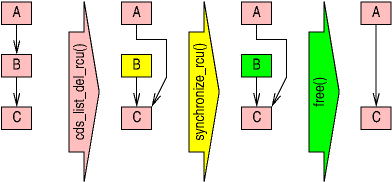
\includegraphics[width=0.7\linewidth]{figures/rcu}
\caption{Ready copy update mechanism, showing deferred destruction \cite{whatisrcu}}
\label{fig:rcu}
\end{figure}
\end{labeling}

Since the introduction of RCU, there have been a lot of improvements. The research from McKenney \emph{et al.} shows that RCU can provide order-of-magnitude speedups for read-mostly data structures \cite{whatisrcu}. RCU is optimal when less than 10\% of accesses are updates over a wide range of CPUs. The work by Sarma \emph{et al.} shows that making RCU suitable for real-time systems relies on improving RCU callbacks and suggests three methods for doing so. The first is to provide per-CPU kernel daemons to process RCU callbacks. Second is to directly invoke the RCU callback and lastly, to throttle the RCU callbacks so that the limited number of callbacks are invoked at a given time \cite{sarma2004making}.

\textbf{Software Transactional Memory:}
Software Transactional Memory (STM) is a concurrency control mechanism that works in a similar way to database transactions by providing atomic and isolated execution for regions of code. The instructions to access shared memory are executed in a transaction, so that the other threads will not see any changes that this thread is making. At the end, either the transaction is committed (if no other threads have modified the data), or aborted (if other threads have modified the data) and the transaction is restarted. 

STM requires language extensions and the compiler takes care of data versioning and conflict detection mechanisms, and makes sure that the global state of the program is consistent. From GCC 4.7, STM support has been added, which makes it ideal to use in this project. Code listing \ref{stm_sample} shows the example transaction execution in GCC.


\begin{lstlisting}[caption={STM example code in GCC},label={stm_sample}, style=customcpp]
void testfunc(int *x, int *y){
_transaction_atomic{
*x += *y;
}
}
\end{lstlisting}

Other nonblocking data structures which are being researched in embedded systems and other operating system groups are, 

\begin{labeling}{waitfree}
\item[\textbf{Wait-free algorithms:}] A wait-free implementation of a concurrent data object guarantees that a thread executes in a finite number of steps, regardless of execution times of other threads  \cite{herlihy1991wait}. For example, when a higher priority thread \textit{A} detects that a lower priority thread \textit{B} is in critical section that it wants to enter, it lends \textit{B} its priority to let \textit{B} finish the execution. When \textit{B} has finished, \textit{A} executes in its own critical section.


\item [\textbf{Lock-free synchronization:}] This method works completely without locks and uses an atomic update operation like Compare-and-Swap(CAS). \textit{Critical code sections are designed such that they prepare their results out of line and then try to commit them to the pool of shared data using an atomic memory update instruction} \cite{hohmuth2001pragmatic}. The CAS works in two steps. The \textit{compare} step detects the conflict between two threads that are updating the memory location. In case of failure, the whole operation is restarted. This gives deadlock a free code, but requires that primitives for atomic memory update operations are available.
\end{labeling}



\section{Evaluation of Synchronization techniques}

\begin{center}
\begin{tabular}{|l|l|l|p{3cm}|}
\hline 
\textbf{Criteria} & \textbf{Mutex} & \textbf{RCU} & \textbf{STM} \\ \hline

Implementation & + & - - & ++ \\ \hline

Read-speed & - - & ++ & + \\ \hline

Write-speed & - - & + & + \\ \hline

Deadlocks & - - & ++ & + \\ \hline

Overhead & + & + & - - \\ \hline

Security/Consistency & ++ & - & + \\ \hline
\end{tabular}
\captionof{table}{ Evaluation of synchronization techniques}\label{tab:lock}
\end{center}

The evaluation of these methods are based on the study of the above mentioned papers and the work of Heaker's analysis. Lock-based methods and STM are easy to implement since the language constructs provide this mechanism. STM is better than locks because with using many locks, the code can become unreadable, whereas the STM code has better readability \cite{pankratius2014software}. RCU is hard to implement, since the developer has to take care of providing all the read side locks, grace period handling and list operations.

RCU is better to use when there are multiple readers, so that the read speed is very good. RCU also has a better write-speed when compared to locks. Locks perform the worst in read and write speed since only one thread can access the data at a time. STM's read and write speed is also good, but the only drawback is that it might have to read again if the data changes in the middle of a transaction.

There is no deadlock problem in RCU, while deadlocks are common in locks. STM also suffers from data races. RCU and locks have less overhead compared to STM. This is because STM has to keep the logs of the transaction and has to take care to roll-back if something goes wrong. The data is consistent at all times while using locks but this is not same for RCU and STM. RCU has multiple versions of the data and STM has logs to keep the old data.

The recent research on STM is increasing. Ferad \emph{et al.}'s research suggests that implementing STM from scratch is better than trying to convert the programs, which use locks to an STM implementation \cite{zyulkyarov2009atomic}. The research by Victor \emph{et al.} \cite{pankratius2014software} showed that STM is a very good tool but needs C++ language refinements and better debugging support, and large transactions can hurt the performance.

RCU seems to be a better choice for providing synchronized access to the ready queue but it adds considerable code, given the fact that it is an embedded system. Testing the lock-based and a lock free algorithm on a real system will provide a better heuristic. 

%\section{System Requirements} \label{foundations_cons}
%Since the system in use is a safety-critical real time system, there are certain factors to be considered in proposing a solution to the system.
%
%\begin{enumerate}
%
%\item Since the system is a safety-critical real time system, the safety becomes major criteria. The system should be in a predictable state always and is able to gracefully handle any error state.
%
%\item Any solution that is proposed should be efficient, since the used system is a embedded system. Since the system contains the less memory and processing power, the code should be simple and efficient.
%
%\item The utilization of the CPU should be intelligent to ensure that the all threads reach their deadline, since the computed value of no use once the deadline has passed. This requires a effective scheduling strategy to be used. 
%
%\end{enumerate}